\chapter*{Experiment 1 - Blink}
\addcontentsline{toc}{chapter}{Experiment 1 - Blink}
This example is what one might call the \textit{hello world} example for \gls{Arduino} sketches. We wire up the experiment as shown in the diagram fig:~\ref{fig:exp1_blink}. And upload the \gls{Sketch} code in the next section on page:~\pageref{sketch:exp1}.

%
\begin{figure}[ht]
	\centering
	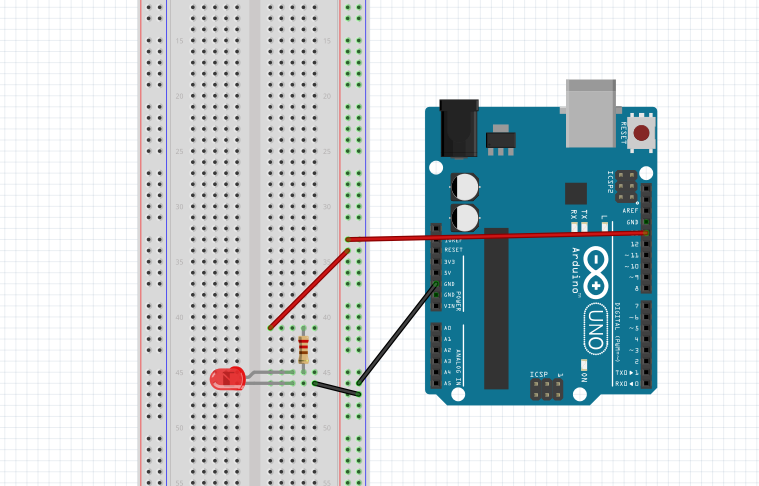
\includegraphics[width=12cm]{images/07}
	\caption{LED Blink \citep{fritzing-15}}
	\label{fig:exp1_blink}
\end{figure}
%

When the Arduino boots, the led should flash on for a second, then off for a second and repeat.

\newpage
\section*{Sketch Code}
\label{sketch:exp1}
\begin{lstlisting}
/*
Blink
Turns on an LED on for one second, then off for one second, repeatedly.

This example code is in the public domain.
*/

// the setup function runs once when you press reset or power the board
void setup() {
  // initialize digital pin 13 as an output.
  pinMode(13, OUTPUT);
}

// the loop function runs over and over again forever
void loop() {
  // turn the LED on 
  // (HIGH is the voltage level)
  digitalWrite(13, HIGH);
	
  //wait for 1000 milliseconds
  delay(1000);
	
  // turn the LED off by making 
  // the voltage LOW
  digitalWrite(13, LOW);    
	            
  // wait for 1000 milliseconds              
  delay(1000);
}
\end{lstlisting}